\chapter{Appendix}

\begin{figure}[H]
    \centering
    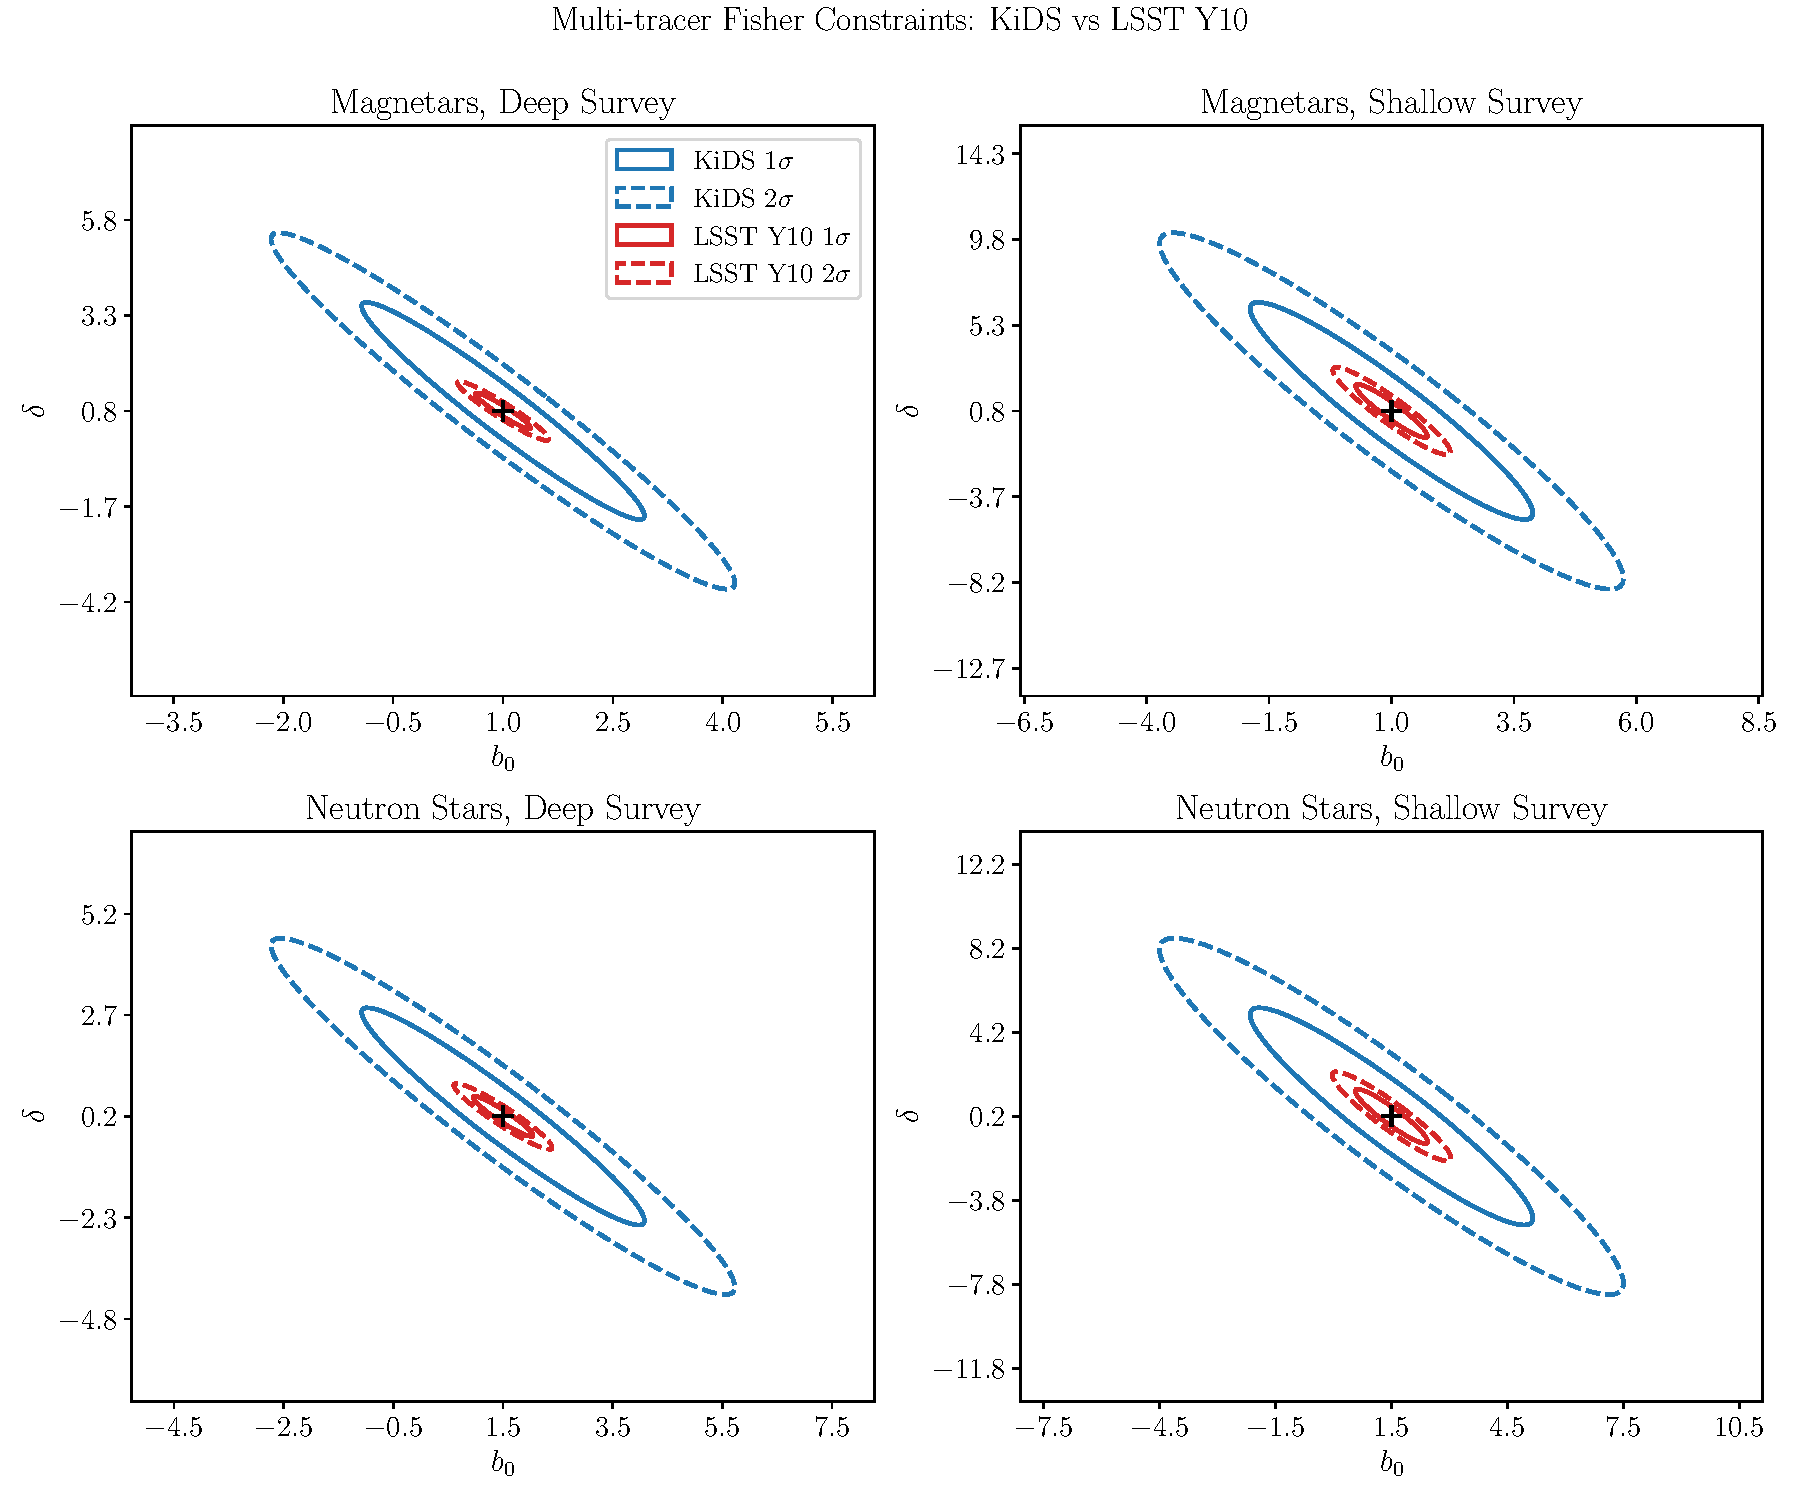
\includegraphics[width=\textwidth]{../programming/frb-cosmology/plots/fisher_lsst/fisher_kids_vs_lsst_2x2.pdf}
    \caption{Comparison of the joint FRB$\times$galaxy forecast for the KiDS-Legacy and LSST Y10
    lens samples, shown for the two progenitor classes and FRB survey configurations.}
    \label{fig:fisher_kids_vs_lsst}
\end{figure}

\begin{table}[H]
    \centering
    \small
    \caption{Marginalized $1\sigma$ errors of the joint FRB$\times$galaxy
    forecast for the two galaxy surveys.}
    \label{tab:lsst_sigmas}
    \begin{tabular}{
        l@{\hspace{1.2em}}
        l@{\hspace{1.2em}}
        S[table-format=1.2]
        @{\hspace{1.4em}}
        S[table-format=1.2]
        @{\hspace{1.4em}}
        S[table-format=1.2]
        @{\hspace{1.2em}}
        S[table-format=1.2]
        }
        \toprule
        & &\multicolumn{2}{c}{$\sigma_{b_0}$}
        & \multicolumn{2}{c}{$\sigma_{\delta}$} \\
        \cmidrule(lr){3-4} \cmidrule(lr){5-6}
        Progenitor class & Configuration
        & {KiDS} & {LSST Y10}
        & {KiDS} & {LSST Y10} \\
        \midrule
        Magnetars     & Deep    & 1.27 & 0.25 & 1.88 & 0.31 \\
        Magnetars     & Shallow & 1.91 & 0.48 & 3.76 & 0.92 \\
        Neutron stars & Deep    & 1.70 & 0.36 & 1.77 & 0.33 \\
        Neutron stars & Shallow & 2.42 & 0.62 & 3.41 & 0.85 \\
        \bottomrule
    \end{tabular}
\end{table}

\begin{table}[H]
    \centering
    \small
    \caption{Figures of merit of the joint FRB$\times$galaxy
    forecast for the two galaxy surveys. The last column gives the ratio
    of the two figures of merit.}
    \label{tab:lsst_fom}
    \begin{tabular}{
        l@{\hspace{0.8em}}
        l@{\hspace{0.4em}}
        S[table-format=1.2]
        @{\hspace{0.2em}}
        S[table-format=2.2]
        @{\hspace{0.4em}}
        S[table-format=2.1]
        }
        \toprule
        & &\multicolumn{3}{c}{FoM}  \\ %
        \cmidrule(lr){3-5}
        Progenitor class & Configuration
        & {KiDS} & {LSST Y10} & {Ratio}\\
        \midrule
        Magnetars     & Deep    & 1.59 & 42.01 & 26.4 \\
        Magnetars     & Shallow & 0.41 &  6.29 & 15.3 \\
        Neutron stars & Deep    & 1.15 & 25.72 & 22.3 \\
        Neutron stars & Shallow & 0.34 &  5.13 & 14.9 \\
        \bottomrule
    \end{tabular}
\end{table}

TABELLEN NOCHMAL ANGUCKEN UND DIE STRICHEN ANPASSEN, DAMIT SIE BESSER ZUSAMMENPASSEN. AUCH DIE SPALTENBREITEN KÖNNTEN NOCHMAL ANGEPASST WERDEN, DAMIT ES BESSER AUSSIEHT.